\chapter{Chapter 2: Perceptual saliencies of subphonemic features}
\section{Introduction}
A common processing malfunction in speech perception is the misperception of one phoneme as another in normal or noisy conditions, usually in the context of spoken words or sentences. For example, when mishearing someone saying ‘take it’ as ‘make it’. Notably, some of phoneme substitutions are more likely than others. For example, putting aside non-phonolgical effects, it is more likely to mishear ‘take it’ as ‘fake it’ than as ‘make it’. One contributing factor for such confusions is that the pair of phonemes /t/-/f/ is more confusable with each other than the pair /t/-/m/. This raises the question: what makes one pair of phonemes more perceptually confusable, or similar \citep{Tversky1977, Shepard1987}, than another pair? Section 2.1.1 provides a brief history of the main developments of phonological theories, described according to two lines of research - auditory and gestural theories. Section 2.1.2 discusses phoneme-similarity theories and the empirical approach to phoneme similarity. Finally, section 2.1.3 presents a new methodological approach to the problem.  

\subsection{Feature theories}
Speech sounds often exhibit the same behavior, grouping together into sound patterns in spoken languages. For example, in German, the singular and plural forms consistently differ by specific pairs of sounds, such as /b/-/p/ in the German word for 'robbery': Raube vs. Raub (final b pronounced as /p/); or for 'bath': /d/-/t/ in  Bäder  vs. Bad (final d pronounced as /t/), and /g/-/k/, /z/-/s/ and /v/-/f/ in other cases. All these different pairs of phonemes have a single property in common: in the plural form, the sounds (/bgdvz/) always include voicing - a vibration of the vocal chords during pronunciation, which has identifiable acoustic markers - whereas in the singular form, the corresponding sounds are unvoiced. Such groups of sounds are termed \textit{natural classes} and they are denoted by subphonemic features, such as [-voice] and [+consonantal]. Natural classes are typically affected, and affect other sounds, in the same way in the same environment, as in the above example. It was therefore suggested that phonological alterations, such as the devoicing process, act on subphonemic features rather than on the phonemic segments themselves. Interestingly, different languages may present similar to identical processes. For example, in Turkish, similarly to German, we find final devoicing in, e.g., 'kitabim' ('my book') vs. 'kitap' ('book'), or 'a\u{g}aim' ('my tree') vs. 'a\u{g}a\c{c}' ('tree'). Such similarities have led to the hypothesis that phonological features are universal and innate (\citealp{ChomskyHalle1968}, but see \citealp{mielke2008emergence}).

\paragraph{Auditory theories}
Around the mid of the 20$^{th}$ century, \citet{jakobson1951preliminaries} suggested that phonological patterns in all languages can be described with only a limited number of contrasting features, such as, voiced-unvoiced, strident-mellow, or nasal-oral. According to this theory, all features can be assigned a unique acoustic correlate, which in turn, correspond to specific articulatory parameters. The articulatory stage, however, is viewed as a mere mechanism to generate acoustic contrasts - "we speak to be heard in order to be understood" (ibid.), and features do not necessarily have a unique articulatory correlate. This line of research, emphasizing the acoustic aspect of distinctive features, was later developed by \textit{the quantal theory of speech perception} \citep{stevens1972quantal,stevens1989quantal}. This theory added to the field by characterizing the interactions between articulatory parameters of speech and their acoustic outcomes. It suggested that the mapping between articulation to acoustics is highly non-linear, with stable regions (small changes in the articulator have small acoustic effects) and unstable regions (small changes in the articulator generate large acoustic effects). The discontinuities around the unstable regions are used to define the boundaries between features. In this way, the theory accounts for a fundamental question in the field - why languages distinctly favor certain articulatory and acoustic dimensions in constructing their phoneme inventories, while avoiding others. The quantal theory explains this by defining optimality of features - a feature is optimal if it maximizes the difference between phonemes in the auditory space while preserving minimal articulatory effort. This phonological economy explains why features are universal, as they are dependent on biological properties of the human speech-production system, which are essentially the same for all humans.

\paragraph{Gestural theories}
From around the middle of the 20$^{th}$ century, a competing view to auditory theories was developed, called {\it The Motor Theory of Speech Perception} \citep{cooper1952some, liberman1967perception}. Its primary motivation stemmed from the observation that acoustic waveforms of synthetic speech have to be modified in order to produce a constant perception of the same phoneme in different phonological contexts. It was therefore concluded that the objects of speech perception cannot be found in acoustics, in contrast to the view of auditory theories, but should rather be anchored in articulatory gestures. Accordingly, during speech perception, the hearer extracts the intended phonetic gestures of the speaker \citep{liberman1985motor}, rather than acoustic cues. Phonemes are thus viewed as groups of gestural features. In a later theory in the same thread of research, giving emphasis to articulation as well, \citet{ChomskyHalle1968} suggested that phonological patterns across languages can be accounted for with an innate set of articulatory features. Importantly, they argue that what is perceived depends not only on the physical constitution of the signal but also on the linguistic knowledge of the hearer, introducing top-down and expectation processes into the field of speech perception. A further development of this line of research, called feature geometry \citep{clements1985, sagey1986representation}, suggested that speech sounds have an internal featural structure, rather than being comprised of a "bundle" of features. In its simple form, the theory describes the internal structure of segments in terms of a tree, whose nodes are features, higher levels are feature classes and, finally, the root node represents the entire object. Describing sounds with trees enabled the theory to account for phonological patterns in a more parsimonious way compared to previous theories. More recently, \citet{browman1990tiers, browman1992articulatory} suggested a model of gestural coordination known as \textit{Articulatory phonology}. Their underlying hypothesis is that spoken language is best described by patterns of coordinated articulatory gestures. The theory proposes to model phonetic and phonological patterns in terms of "articulatory scores", which are formal representations consisting of abstract gestures and their patterns of coordination.


\subsection{Theories for phoneme similarity}
\paragraph{Feature-based approach}
Phoneme similarity is traditionally explained by decomposing phonemes into subphonemic features, assuming the more features two phonemes share the more similar they are \citep{Tversky1977, Shepard1987, Cohen2009, Cohen2010}. Given a feature theory, a metric (distance) or a phoneme-similarity functions can be defined over pairs of phonemes. For example, given the three contrastive articulatory dimensions - voicing, place- and manner-of-articulation - a common similarity function in psycholinguistics is to count the number of dimensions on which two phonemes agree (e.g., \citealp{mcmillan2010cascading, Bailey2005, mousikou2015masked}). For instance, the phoneme /b/ is labial-plosive-voiced, and the phoneme /g/ is velar-plosive-voiced. The similarity score for these two phonemes is thus two. Other, more sophisticated, similarity measures have been proposed in the literature. These include a similarity measure based on the number of shared and non-shared features \citep{Pierrehumbert1993}, or on the number of shared and non-shared natural classes \citep{Frisch1997}. According to this last measure, similarity between two phonemes is the proportion of natural classes that are shared by the two phonemes, compared to the total shared and not-shared natural classes. Features are thus assigned weights according to their redundancy. Therefore, different features contribute differently in explaining perceptual distances, since redundant features affect similarity less than non-redundant features.

\paragraph{Experimental approach}
Another approach to phoneme similarity addresses the problem by quantifying perceptual phoneme similarities directly in an experiment. Typically, such experiments present noise-corrupted phonemes to subjects, collecting their perceptual judgments of phoneme identity \citep{NicelyMiller1955}. Confusion matrices are then derived from the data, mapping the likelihood that any given phoneme is confused with another phoneme. This approach has been widely used, however, there are several associated concerns that should be kept in mind. First, phoneme confusions may depend on the noise characteristics added to the signal. For example, results from phoneme-confusion experiments using white noise (e.g., \citealp{NicelyMiller1955, Luce1987}) may differ from those that use pink noise (e.g., \citealp{redford1999relative}), or speech-shaped ('babble') noise \citep{cutler2004patterns}. Another source of variability is due to context effects. These may have large effects on perceptual confusability, in particular, consonant confusions may be different when the consonant is in initial or final position of the word \citep{Luce1987, hura1992role, redford1999relative}. Finally, phoneme perception shows asymmetric effect \citep{kuhl1991human}, which was addressed by several feature theories. For example, the featurally underspecified lexicon (FUL) theory \citep{lahiri2002underspecified, lahiri2010distinctive} accounts for asymmetry effects by stating that some features are universally underspecified. For instance, the feature [coronal] is underspecified in the lexicon, which prevents mismatches between labial or dorsal sounds that are detected in the signal, and allows them to access the lexicon. In contrast, labial and dorsal features are specified, and so a coronal sound detected in the signal will mismatch both of these features, and cannot access the lexicon. In speech production, \citet{Frisch1997} claims that similarity neighborhoods in the mental lexicon affect asymmetries in sound substitutions.

\subsection{A metric-learning approach}
We now describe a general framework that we suggest as a new methodological approach to the problem of phoneme similarity. The approach allows the integration of various effects, such as context or asymmetry, into its framework, and is compatible with various feature theories - e.g., auditory or gestural, and with any choice of noise characteristics in phoneme-confusion experiments - white, pink or speech-shaped.

Traditionally, feature-based theories, such as the ones described above, craft a similarity or a metric function based on theoretical insights and intuition. However, current theoretical metrics do not fully account for empirical perceptual distances (e.g. \citealp{Bailey2005}). One reason for this may be that theoretical metrics misevaluate or underestimate the difference in contribution of each subphonemic feature to perceptual distances. 

In this study, we explore an approach that learns a metric function directly from the data, assuming only its general form. For this, we parametrize a general metric function and derive its values using learning algorithms. A geometric interpretation of this approach is illustrated in figure 2.1. Given a feature theory, phonemes can be represented as points in feature space, in which dimensions correspond to subphonemic features (figure 2.1 left). The set of all Euclidean distances between phonemes in this space likely differ from the set of the empirical ones (figure 2.1 right), which were derived from, e.g., a phoneme-confusion data. Given this discrepancy between the two structures, we look for an optimal mapping between the two spaces, such that the distances from the feature space will match as closely as possible the set of distances from the experiment (figure 2.1 middle arrow). This optimal mapping defines a metric function over pairs of phonemes. Importantly, once the optimal mapping is derived from the data, one can learn about the perceptually discriminative power of the various features. As an example, if the mapping is linear and represented by a (positive) diagonal matrix, the mapping amounts to stretchings or contractions of the feature dimensions. Dimensions that are relatively highly stretched would thus correspond to features that are more perceptually discriminative.

\begin{figure}
\vspace{.3in}
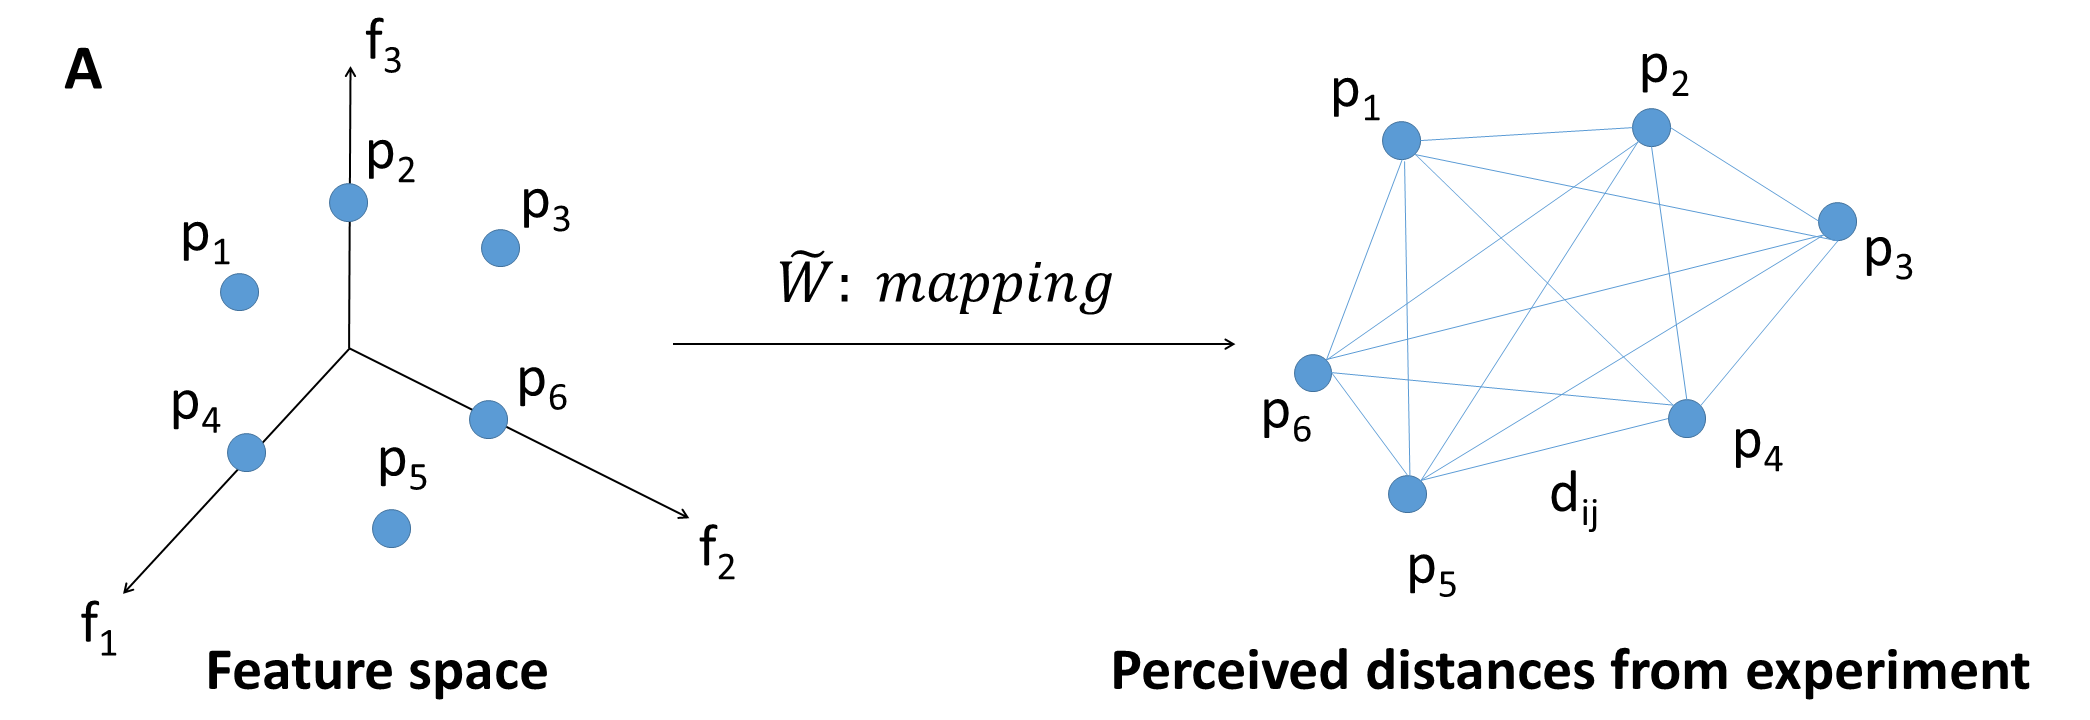
\includegraphics[width=\linewidth]{Figures/Ch2/Figure1_2017Sep10.png}
\caption{An illustration of metric learning for phonemes: phonemes $p_i's$ are represented in a feature space (left), where each dimension corresponds to a feature. Perceptual distances as collected in an experiment $d_{ij}$ (right) are used to learn an optimal mapping (middle arrow), defined over the feature space. The mapping is optimal in the sense that it maps the phonemes from the feature space such that the distances between the mapped phonemes are as close as possible to the empirical ones.}
\end{figure}

We test our approach on two English phoneme-confusion datasets \citep{NicelyMiller1955, Luce1987} and a new dataset that we have collected for Hebrew. In all cases, we focus on consonant confusions at initial position and white noise in all experiments. In addition, we present and compare several alternatives to learn the metric function. For computational convenience, we assume a linear mapping and a symmetric metric function. However, the approach can be pursued with a removal of such assumptions, as we later discuss.